\item O gancho está preso a uma corda que está enrolada em torno do tambor. Se ele se desloca do repouso com uma aceleração de $\SI{6}{\meter/\second^{2}}$, determine a aceleração angular do tambor e sua velocidade angular após o tambor ter completado 10 revoluções. Quantas revoluções mais o tambor realizará após ele ter completado as 10 primeiras e o gancho continuar a se deslocar para baixo por 4 segundos?

\import{../answers/}{answer-1}

\vspace{-2.8cm}
\begin{flushright}
	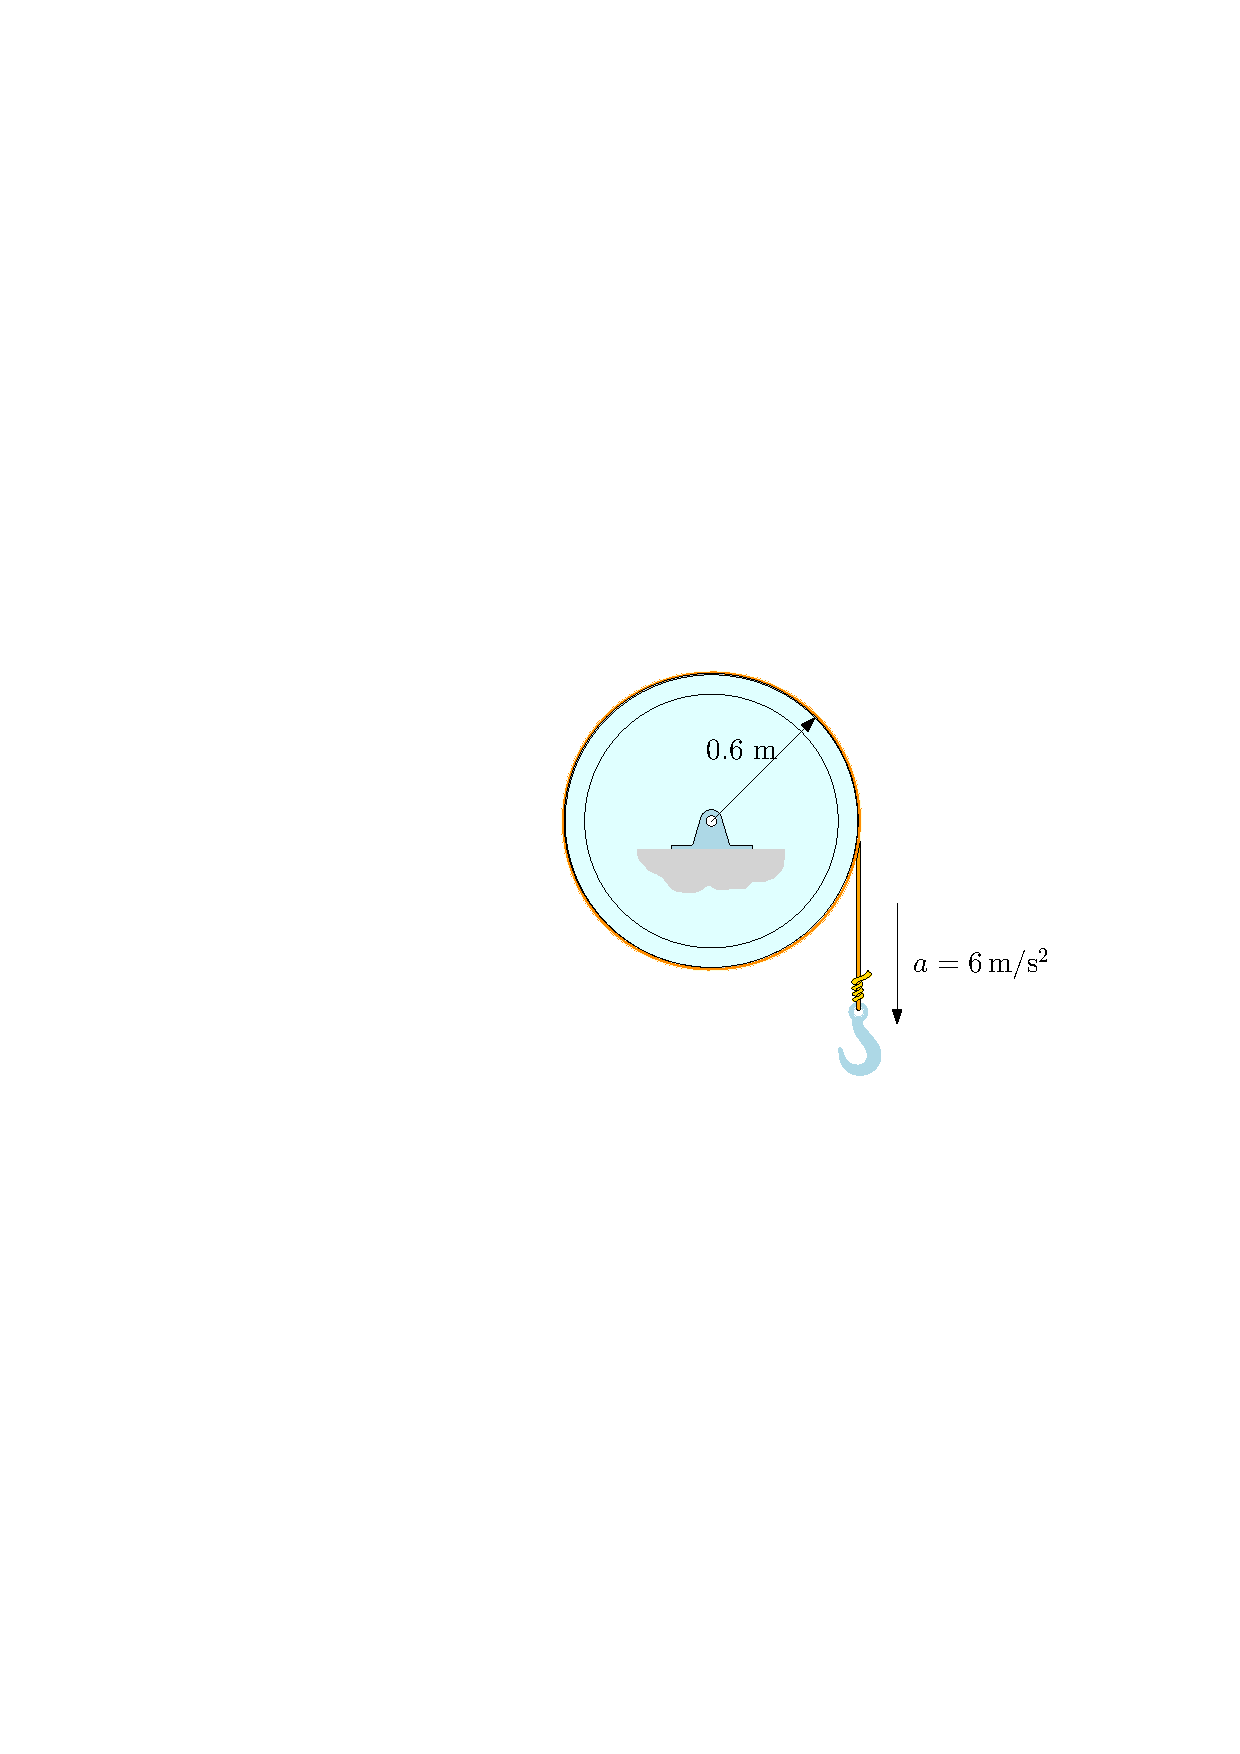
\includegraphics[scale=1]{images/draw_1}
\end{flushright}